% The birth exchange. Right: the default tree B (top) and its birth-exchanged tree B_Ex (bottom),
% joined by a bijection arrow. Left: the same tree with the labelling forgotten, as in Figure 1a of
% Paper01_AgeBDPVarEnv/AgeBDP.tex: at every birth the parent's stem meets the middle of the
% horizontal line and the two children leave from its two ends.
% Coordinates of B follow tree_contour.tex and those of B_Ex the bottom of exchanged_pair.tex.
% Compile with: lualatex "\def\stage{1}% The birth exchange. Right: the default tree B (top) and its birth-exchanged tree B_Ex (bottom),
% joined by a bijection arrow. Left: the same tree with the labelling forgotten, as in Figure 1a of
% Paper01_AgeBDPVarEnv/AgeBDP.tex: at every birth the parent's stem meets the middle of the
% horizontal line and the two children leave from its two ends.
% Coordinates of B follow tree_contour.tex and those of B_Ex the bottom of exchanged_pair.tex.
% Compile with: lualatex "\def\stage{1}% The birth exchange. Right: the default tree B (top) and its birth-exchanged tree B_Ex (bottom),
% joined by a bijection arrow. Left: the same tree with the labelling forgotten, as in Figure 1a of
% Paper01_AgeBDPVarEnv/AgeBDP.tex: at every birth the parent's stem meets the middle of the
% horizontal line and the two children leave from its two ends.
% Coordinates of B follow tree_contour.tex and those of B_Ex the bottom of exchanged_pair.tex.
% Compile with: lualatex "\def\stage{1}% The birth exchange. Right: the default tree B (top) and its birth-exchanged tree B_Ex (bottom),
% joined by a bijection arrow. Left: the same tree with the labelling forgotten, as in Figure 1a of
% Paper01_AgeBDPVarEnv/AgeBDP.tex: at every birth the parent's stem meets the middle of the
% horizontal line and the two children leave from its two ends.
% Coordinates of B follow tree_contour.tex and those of B_Ex the bottom of exchanged_pair.tex.
% Compile with: lualatex "\def\stage{1}\input{birth_exchange.tex}"
\documentclass[tikz,border=4pt]{standalone}
\usepackage{xcolor}
\usepackage{libertinus-otf}
\usepackage{unicode-math}
\setmathfont{STIX Two Math}
\definecolor{paper}{HTML}{FAFAFA}
\definecolor{treecol}{HTML}{D55E00}

% Axes, the terminal level T and a caption, in the local coordinates of one tree.
\newcommand{\treeaxes}[1]{%
  \draw[->] (0,0) -- (22,0) node[right] {$s$};
  \draw[->] (0,0) -- (0,6) node[above] {$t$};
  \draw[dashed, gray] (0,5) -- (22,5);
  \node[left] at (0,5) {$T$};
  \node[left] at (0,0) {$0$};
  \node at (11,6.7) {#1};}

\begin{document}
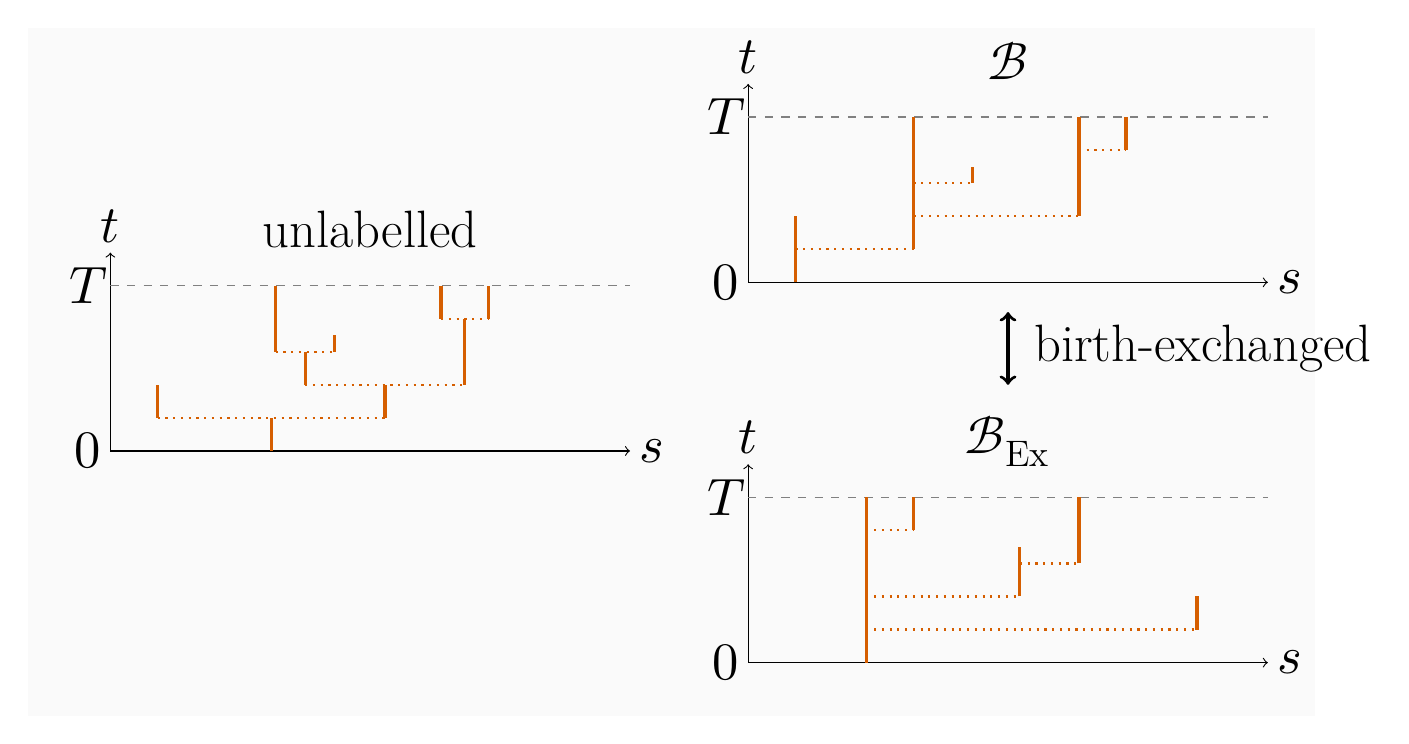
\begin{tikzpicture}[xscale=0.30, yscale=0.42, font=\fontsize{19pt}{23pt}\selectfont]
  \fill[paper] (-3.5,-1.6) rectangle (51,19.2);

  % ---- Left: the unlabelled tree, parent stems at the middle of each birth line ----------
  \begin{scope}[shift={(0,6.4)}]
    \treeaxes{unlabelled}
    \draw[very thick, treecol]
      (6.8125,0) -- (6.8125,1)          % root stem, into the first birth
      (2,1) -- (2,2)                    % left child, dies
      (11.625,1) -- (11.625,2)          % right child, into the second birth
      (8.25,2) -- (8.25,3)              % left child, into the third birth
      (15,2) -- (15,4)                  % right child, into the fourth birth
      (7,3) -- (7,5)                    % survives to T
      (9.5,3) -- (9.5,3.5)              % dies
      (14,4) -- (14,5) (16,4) -- (16,5);
    \draw[thick, treecol, dotted]
      (2,1) -- (11.625,1) (8.25,2) -- (15,2) (7,3) -- (9.5,3) (14,4) -- (16,4);
  \end{scope}

  % ---- Right, top: the tree B -------------------------------------------------------
  \begin{scope}[shift={(27,11.5)}]
    \treeaxes{$\mathcal{B}$}
    \draw[very thick, treecol]
      (2,0) -- (2,2) (7,1) -- (7,5) (14,2) -- (14,5) (9.5,3) -- (9.5,3.5) (16,4) -- (16,5);
    \draw[thick, treecol, dotted]
      (2,1) -- (7,1) (7,2) -- (14,2) (7,3) -- (9.5,3) (14,4) -- (16,4);
  \end{scope}

  % ---- Right, bottom: the birth-exchanged tree B_Ex ---------------------------------
  \begin{scope}[shift={(27,0)}]
    \treeaxes{$\mathcal{B}_{\mathrm{Ex}}$}
    \draw[very thick, treecol]
      (5,0) -- (5,5) (7,4) -- (7,5) (11.5,2) -- (11.5,3.5) (14,3) -- (14,5) (19,1) -- (19,2);
    \draw[thick, treecol, dotted]
      (5,4) -- (7,4) (5,2) -- (11.5,2) (11.5,3) -- (14,3) (5,1) -- (19,1);
  \end{scope}

  % ---- The bijection ------------------------------------------------------------------
  \draw[<->, very thick] (38,8.4) -- (38,10.6);
  \node[anchor=west] at (38.7,9.5) {birth-exchanged};
\end{tikzpicture}
\end{document}
"
\documentclass[tikz,border=4pt]{standalone}
\usepackage{xcolor}
\usepackage{libertinus-otf}
\usepackage{unicode-math}
\setmathfont{STIX Two Math}
\definecolor{paper}{HTML}{FAFAFA}
\definecolor{treecol}{HTML}{D55E00}

% Axes, the terminal level T and a caption, in the local coordinates of one tree.
\newcommand{\treeaxes}[1]{%
  \draw[->] (0,0) -- (22,0) node[right] {$s$};
  \draw[->] (0,0) -- (0,6) node[above] {$t$};
  \draw[dashed, gray] (0,5) -- (22,5);
  \node[left] at (0,5) {$T$};
  \node[left] at (0,0) {$0$};
  \node at (11,6.7) {#1};}

\begin{document}
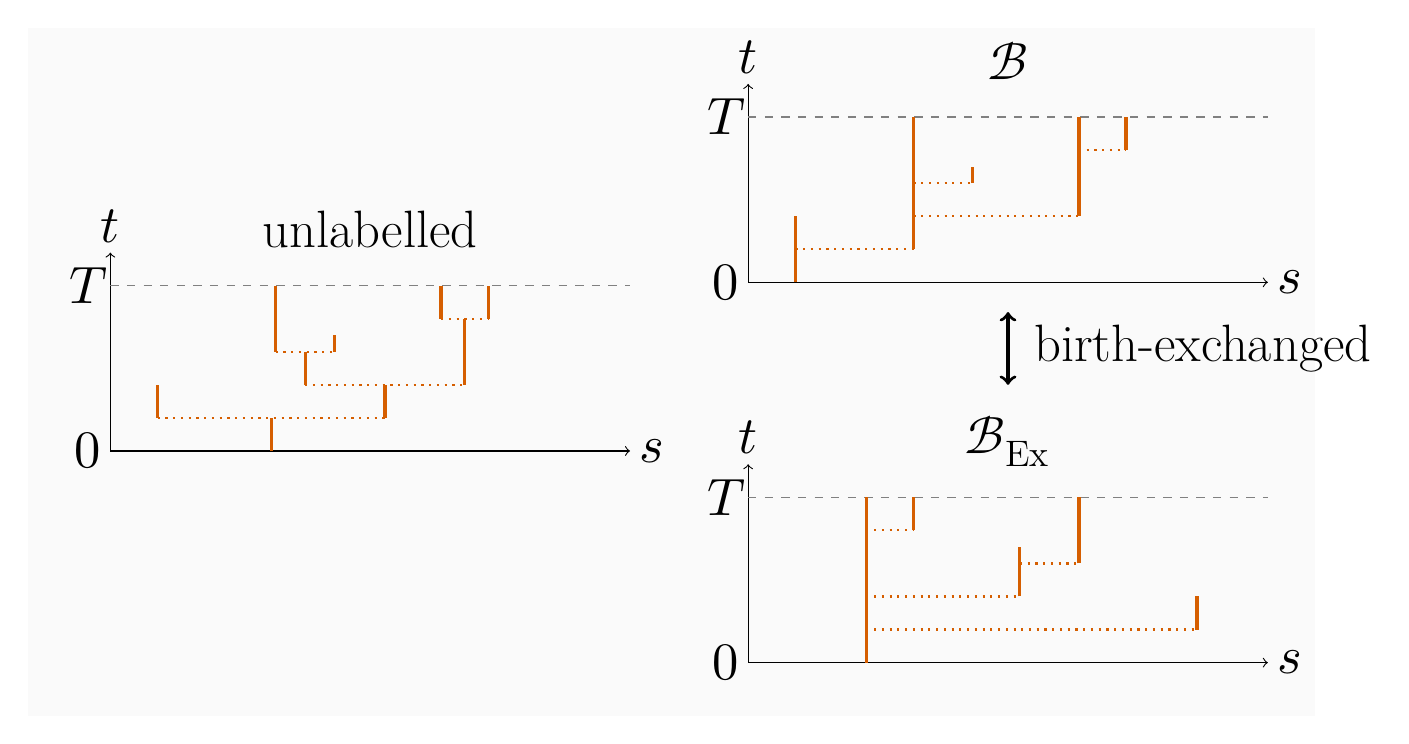
\begin{tikzpicture}[xscale=0.30, yscale=0.42, font=\fontsize{19pt}{23pt}\selectfont]
  \fill[paper] (-3.5,-1.6) rectangle (51,19.2);

  % ---- Left: the unlabelled tree, parent stems at the middle of each birth line ----------
  \begin{scope}[shift={(0,6.4)}]
    \treeaxes{unlabelled}
    \draw[very thick, treecol]
      (6.8125,0) -- (6.8125,1)          % root stem, into the first birth
      (2,1) -- (2,2)                    % left child, dies
      (11.625,1) -- (11.625,2)          % right child, into the second birth
      (8.25,2) -- (8.25,3)              % left child, into the third birth
      (15,2) -- (15,4)                  % right child, into the fourth birth
      (7,3) -- (7,5)                    % survives to T
      (9.5,3) -- (9.5,3.5)              % dies
      (14,4) -- (14,5) (16,4) -- (16,5);
    \draw[thick, treecol, dotted]
      (2,1) -- (11.625,1) (8.25,2) -- (15,2) (7,3) -- (9.5,3) (14,4) -- (16,4);
  \end{scope}

  % ---- Right, top: the tree B -------------------------------------------------------
  \begin{scope}[shift={(27,11.5)}]
    \treeaxes{$\mathcal{B}$}
    \draw[very thick, treecol]
      (2,0) -- (2,2) (7,1) -- (7,5) (14,2) -- (14,5) (9.5,3) -- (9.5,3.5) (16,4) -- (16,5);
    \draw[thick, treecol, dotted]
      (2,1) -- (7,1) (7,2) -- (14,2) (7,3) -- (9.5,3) (14,4) -- (16,4);
  \end{scope}

  % ---- Right, bottom: the birth-exchanged tree B_Ex ---------------------------------
  \begin{scope}[shift={(27,0)}]
    \treeaxes{$\mathcal{B}_{\mathrm{Ex}}$}
    \draw[very thick, treecol]
      (5,0) -- (5,5) (7,4) -- (7,5) (11.5,2) -- (11.5,3.5) (14,3) -- (14,5) (19,1) -- (19,2);
    \draw[thick, treecol, dotted]
      (5,4) -- (7,4) (5,2) -- (11.5,2) (11.5,3) -- (14,3) (5,1) -- (19,1);
  \end{scope}

  % ---- The bijection ------------------------------------------------------------------
  \draw[<->, very thick] (38,8.4) -- (38,10.6);
  \node[anchor=west] at (38.7,9.5) {birth-exchanged};
\end{tikzpicture}
\end{document}
"
\documentclass[tikz,border=4pt]{standalone}
\usepackage{xcolor}
\usepackage{libertinus-otf}
\usepackage{unicode-math}
\setmathfont{STIX Two Math}
\definecolor{paper}{HTML}{FAFAFA}
\definecolor{treecol}{HTML}{D55E00}

% Axes, the terminal level T and a caption, in the local coordinates of one tree.
\newcommand{\treeaxes}[1]{%
  \draw[->] (0,0) -- (22,0) node[right] {$s$};
  \draw[->] (0,0) -- (0,6) node[above] {$t$};
  \draw[dashed, gray] (0,5) -- (22,5);
  \node[left] at (0,5) {$T$};
  \node[left] at (0,0) {$0$};
  \node at (11,6.7) {#1};}

\begin{document}
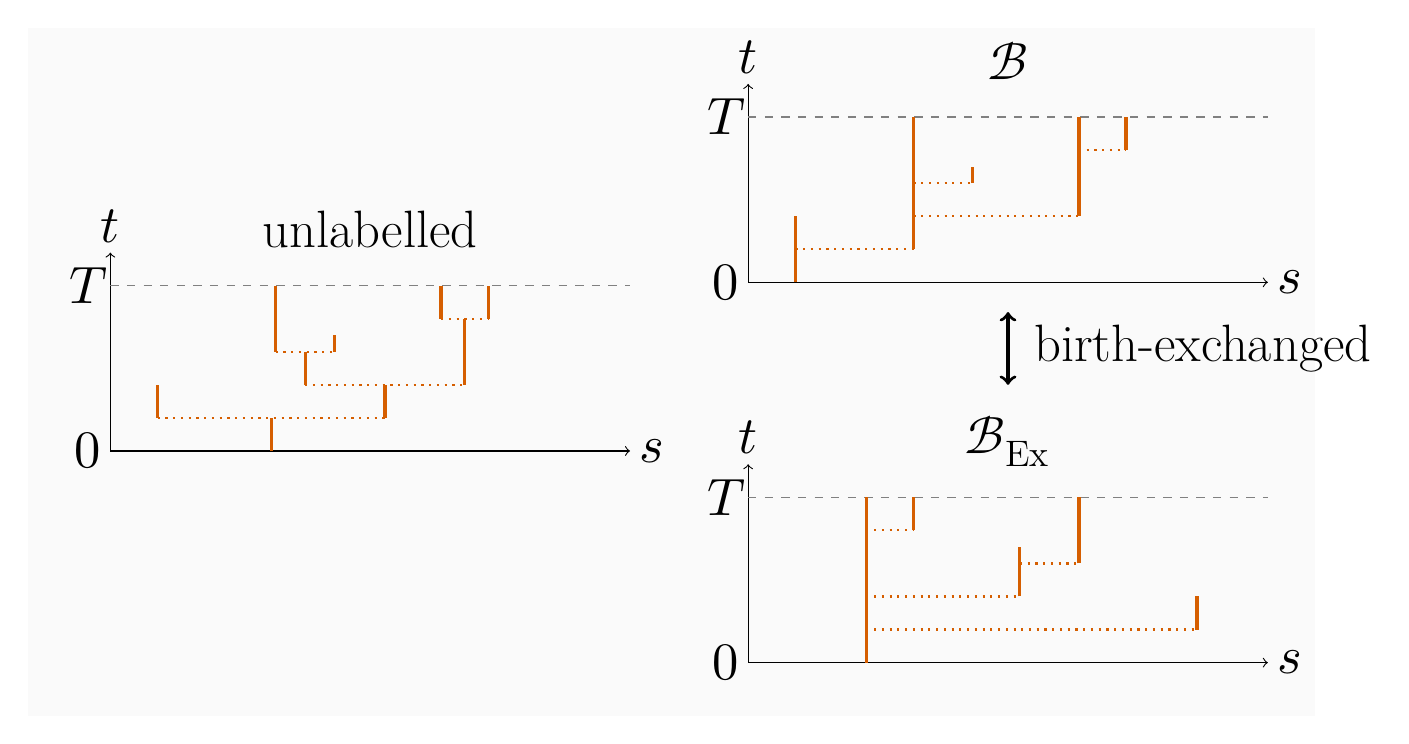
\begin{tikzpicture}[xscale=0.30, yscale=0.42, font=\fontsize{19pt}{23pt}\selectfont]
  \fill[paper] (-3.5,-1.6) rectangle (51,19.2);

  % ---- Left: the unlabelled tree, parent stems at the middle of each birth line ----------
  \begin{scope}[shift={(0,6.4)}]
    \treeaxes{unlabelled}
    \draw[very thick, treecol]
      (6.8125,0) -- (6.8125,1)          % root stem, into the first birth
      (2,1) -- (2,2)                    % left child, dies
      (11.625,1) -- (11.625,2)          % right child, into the second birth
      (8.25,2) -- (8.25,3)              % left child, into the third birth
      (15,2) -- (15,4)                  % right child, into the fourth birth
      (7,3) -- (7,5)                    % survives to T
      (9.5,3) -- (9.5,3.5)              % dies
      (14,4) -- (14,5) (16,4) -- (16,5);
    \draw[thick, treecol, dotted]
      (2,1) -- (11.625,1) (8.25,2) -- (15,2) (7,3) -- (9.5,3) (14,4) -- (16,4);
  \end{scope}

  % ---- Right, top: the tree B -------------------------------------------------------
  \begin{scope}[shift={(27,11.5)}]
    \treeaxes{$\mathcal{B}$}
    \draw[very thick, treecol]
      (2,0) -- (2,2) (7,1) -- (7,5) (14,2) -- (14,5) (9.5,3) -- (9.5,3.5) (16,4) -- (16,5);
    \draw[thick, treecol, dotted]
      (2,1) -- (7,1) (7,2) -- (14,2) (7,3) -- (9.5,3) (14,4) -- (16,4);
  \end{scope}

  % ---- Right, bottom: the birth-exchanged tree B_Ex ---------------------------------
  \begin{scope}[shift={(27,0)}]
    \treeaxes{$\mathcal{B}_{\mathrm{Ex}}$}
    \draw[very thick, treecol]
      (5,0) -- (5,5) (7,4) -- (7,5) (11.5,2) -- (11.5,3.5) (14,3) -- (14,5) (19,1) -- (19,2);
    \draw[thick, treecol, dotted]
      (5,4) -- (7,4) (5,2) -- (11.5,2) (11.5,3) -- (14,3) (5,1) -- (19,1);
  \end{scope}

  % ---- The bijection ------------------------------------------------------------------
  \draw[<->, very thick] (38,8.4) -- (38,10.6);
  \node[anchor=west] at (38.7,9.5) {birth-exchanged};
\end{tikzpicture}
\end{document}
"
\documentclass[tikz,border=4pt]{standalone}
\usepackage{xcolor}
\usepackage{libertinus-otf}
\usepackage{unicode-math}
\setmathfont{STIX Two Math}
\definecolor{paper}{HTML}{FAFAFA}
\definecolor{treecol}{HTML}{D55E00}

% Axes, the terminal level T and a caption, in the local coordinates of one tree.
\newcommand{\treeaxes}[1]{%
  \draw[->] (0,0) -- (22,0) node[right] {$s$};
  \draw[->] (0,0) -- (0,6) node[above] {$t$};
  \draw[dashed, gray] (0,5) -- (22,5);
  \node[left] at (0,5) {$T$};
  \node[left] at (0,0) {$0$};
  \node at (11,6.7) {#1};}

\begin{document}
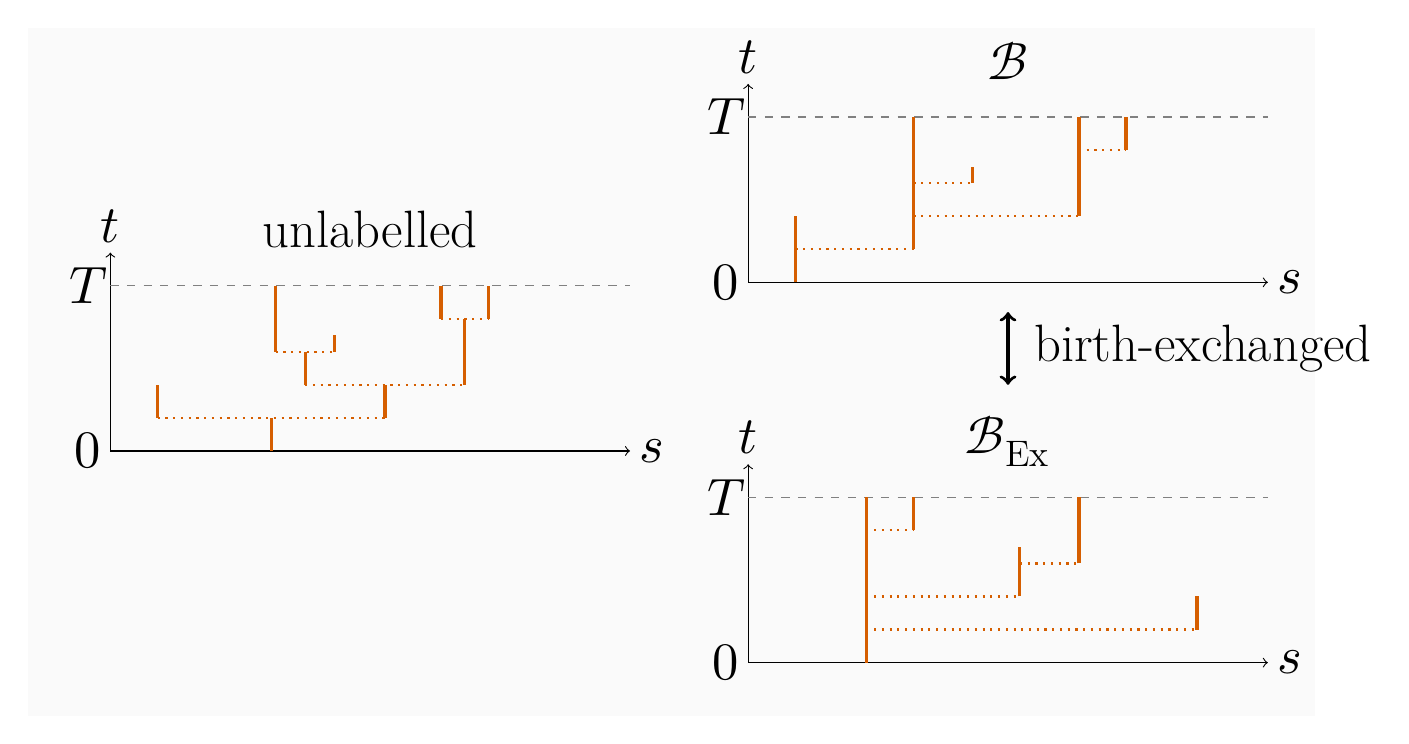
\begin{tikzpicture}[xscale=0.30, yscale=0.42, font=\fontsize{19pt}{23pt}\selectfont]
  \fill[paper] (-3.5,-1.6) rectangle (51,19.2);

  % ---- Left: the unlabelled tree, parent stems at the middle of each birth line ----------
  \begin{scope}[shift={(0,6.4)}]
    \treeaxes{unlabelled}
    \draw[very thick, treecol]
      (6.8125,0) -- (6.8125,1)          % root stem, into the first birth
      (2,1) -- (2,2)                    % left child, dies
      (11.625,1) -- (11.625,2)          % right child, into the second birth
      (8.25,2) -- (8.25,3)              % left child, into the third birth
      (15,2) -- (15,4)                  % right child, into the fourth birth
      (7,3) -- (7,5)                    % survives to T
      (9.5,3) -- (9.5,3.5)              % dies
      (14,4) -- (14,5) (16,4) -- (16,5);
    \draw[thick, treecol, dotted]
      (2,1) -- (11.625,1) (8.25,2) -- (15,2) (7,3) -- (9.5,3) (14,4) -- (16,4);
  \end{scope}

  % ---- Right, top: the tree B -------------------------------------------------------
  \begin{scope}[shift={(27,11.5)}]
    \treeaxes{$\mathcal{B}$}
    \draw[very thick, treecol]
      (2,0) -- (2,2) (7,1) -- (7,5) (14,2) -- (14,5) (9.5,3) -- (9.5,3.5) (16,4) -- (16,5);
    \draw[thick, treecol, dotted]
      (2,1) -- (7,1) (7,2) -- (14,2) (7,3) -- (9.5,3) (14,4) -- (16,4);
  \end{scope}

  % ---- Right, bottom: the birth-exchanged tree B_Ex ---------------------------------
  \begin{scope}[shift={(27,0)}]
    \treeaxes{$\mathcal{B}_{\mathrm{Ex}}$}
    \draw[very thick, treecol]
      (5,0) -- (5,5) (7,4) -- (7,5) (11.5,2) -- (11.5,3.5) (14,3) -- (14,5) (19,1) -- (19,2);
    \draw[thick, treecol, dotted]
      (5,4) -- (7,4) (5,2) -- (11.5,2) (11.5,3) -- (14,3) (5,1) -- (19,1);
  \end{scope}

  % ---- The bijection ------------------------------------------------------------------
  \draw[<->, very thick] (38,8.4) -- (38,10.6);
  \node[anchor=west] at (38.7,9.5) {birth-exchanged};
\end{tikzpicture}
\end{document}
